% !TEX root = ./informe.tex

\section{Problema 2}

\subsection{Explicación}

El contexto del problema es el siguiente: tenemos un conjunto de ciudades conectadas por rutas con peajes. El costo de un peaje es cuanto se debe pagar por transitar la ruta, y el mismo puede ser negativo (uno en vez de pagar por pasar, cobra). Decimos que hay un `abuso' si podemos partir de una ciudad $c$ arbitraria y volver, teniendo un saldo positivo de dinero. El problema es encontrar el máximo $K$ que le puedo restar a todos los peajes sin que haya ningún abuso. \\

Notemos que podemos considerar a las ciudades como nodos, a las rutas como aristas, y a los peajes como el peso de las mismas; modelando el contexto como un grafo. Visto esto, el problema se reduce a encontrar el máximo $K$ tal que en el grafo original con todos los pesos decrementados en $K$, no haya circuito simples negativos. \\

Veamos un ejemplo: \\

\vspace{0.1cm}

{\centering
  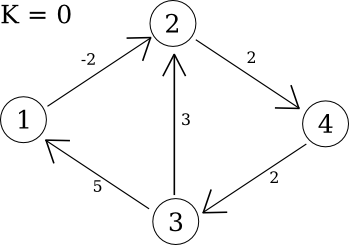
\includegraphics[width=0.50\textwidth]{imagenes/problema2/prob2_caso3.png} \\
  \captionof{figure}{Ningún ciclo es negativo}
}
$ $\newline

\begin{figure}[H]
	\centering
	\begin{minipage}[b]{0.45\textwidth}
		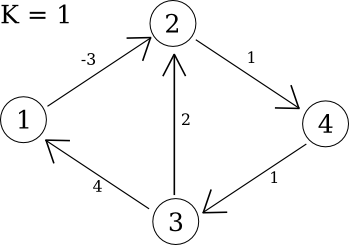
\includegraphics[width=\textwidth]{imagenes/problema2/prob2_caso3_c1.png} \\
		\captionof{figure}{Ningún ciclo es negativo}
	\end{minipage}
	\hfill
	\begin{minipage}[b]{0.45\textwidth}
		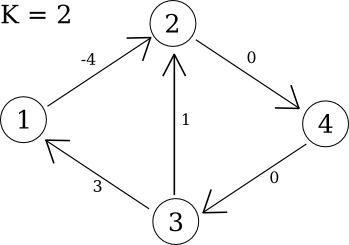
\includegraphics[width=\textwidth]{imagenes/problema2/prob2_caso3_c2.png} \\
		\captionof{figure}{
			Existe ciclo que suma negativo: $0 + 0 + 3 -4 = -1$
		}
	\end{minipage}
\end{figure}

Para cada $K$, los costos de cada arista disminuyen en $K$ con respecto al grafo inicial. Queremos encontrar el máximo $K$ tal que la suma de los costos de los peajes de todos los ciclos no sea negativa. En otras palabras, queremos encontrar el máximo $K$ tal que no se formen ciclos negativos. Observamos que con $K = 2$ existe un ciclo negativo si pasamos por los nodos 1-2-4-3-1, pero no existe ningun ciclo negativo con $K = 1$. Por lo tanto, el valor máximo (y respuesta final) en este ejemplo es $1$. \\


\subsection{Correctitud}

La noción de \textit{abuso} en un grafo se corresponde con la existencia de ciclos negativos. Por esta razón, para resolver el problema querremos ser capaces de responder si un grafo tiene ciclos negativos o no. \\

El algoritmo de Bellman Ford es capaz de detectar si hay un ciclo negativo entre dos nodos. Sin embargo, notemos que la ausencia de ciclos negativos entre dos nodos no necesariamente implica que no exista uno en el grafo entero. Esto puede ocurrir porque no se nos garantiza que la entrada forme un grafo orientado fuertemente conexo, por lo que podríamos llegar a tener un ciclo negativo cuyos nodos no sean alcanzables por el nodo con el que arrancamos el algoritmo. \\

Para solucionar esto, vamos a extender nuestro grafo de entrada con un nuevo nodo $u$ con una arista hacia todos los demás nodos. De esta forma, todos los nodos (y por ende los posibles ciclos negativos) serán alcanzables desde $u$. Desde ese nodo, aplicando Bellman Ford podremos ver la existencia de ciclos negativos en cualquier parte del grafo. Como solo estaríamos agregando aristas de ida desde un nuevo nodo, no agregaríamos nuevos ciclos entre los nodos ya existentes. Lo que estaríamos obteniendo al final, es si nuestro grafo original presenta un abuso, o no lo presentaba. \\

Esto nos da una forma de detectar abuso en grafos. Ahora, lo que pide el enunciado es encontrar el máximo valor por el cual puedo decrementar el peso de todos los ejes sin que haya abuso. Lo que vamos a hacer es una suerte de búsqueda binaria sobre el rango $[0..c+2)$. \\

Veamos primero que el $k$ que buscamos se encuentra en ese rango. No puede ser negativo, porque estamos buscando un máximo, y porque en la entrada no tenemos abuso, lo que implica que el $0$ ya es posible candidato a solución. Tampoco puede ser mayor a $c+1$ , porque como $c$ es el máximo costo, quedarían todos los costos de los peajes negativos. Por el enunciado, sabemos que todas las ciudades tienen una ruta de salida, con lo cual siempre podemos asegurar que existe al menos un ciclo. Si todos los peajes son negativos, esto implica que nos quedaría algún ciclo negativo. \\

¿Cómo hacemos la búsqueda binaria? En cada iteración tomamos el valor $m$ a la mitad de nuestro espacio de búsqueda, y preguntamos si nuestro grafo con los pesos decrementados en $m$ presenta abuso. Si hay, entonces sabemos que nuestro $k$ no es $m$; y que si ya con $m$ tenemos un abuso, con valores mayores lo seguiremos teniendo. Por ende, puedo descartar a $m$ y a la mitad superior de nuestro espacio de búsqueda. Si por el contrario, restando $m$ no nos da un abuso, entonces $m$ es un posible candidato a $k$. Como busco un máximo, puedo descartar la mitad inferior de nuestro espacio de búsqueda. Entonces, lo que estaríamos buscando efectivamente sería el máximo $k$ tal que no hay abuso en el grafo producto de haber decrementado todos los pesos de los ejes en $k$. \\

\newpage
\subsection{Pseudocódigo}

Vamos a utilizar como entrada en nuestro algoritmo las siguientes variables:
\begin{itemize}
	\item $n$: La cantidad de ciudades.
	\item $grafo$: El grafo de entrada representado con listas de adyacencia. Las posiciones del $1$ a $n$ representan nuestras ciudades, mientras que la posición $0$ se deja libre para la extensión.
	\item $costo$: La matriz con los costos de peaje, en donde en la posición $(i,j)$ está el costo de la ruta que va desde $i$ hasta $j$.
	\item $c$: El máximo costo de peaje.
\end{itemize}

\begin{algorithm}[H]
% \label{ej2}         % and a label for \ref{} commands later in the document
\begin{algorithmic}
\Function{Resolver}{}    \Comment{$\mathbf{\mathcal{O}(log \, c*n*\sum_{v \in G} d(v))}$}
	\State ExtenderGrafo()    \Comment{$\mathcal{O}(n)$}
    \State $d \gets 0$    \Comment{$\mathcal{O}(1)$}
	\State $h \gets c + 2$    \Comment{$\mathcal{O}(1)$}
	\While{$h - d > 1$}    \Comment{$\mathcal{O}(log \, c)$}
		\State $mid \gets (h + d)/2$    \Comment{$\mathcal{O}(1)$}
		\If{$\neg$HayAbuso($mid$)}    \Comment{$\mathcal{O}(n*\sum_{v \in G} d(v))$}
			\State $d \gets mid$    \Comment{$\mathcal{O}(1)$}
		\Else
			\State $h \gets mid$    \Comment{$\mathcal{O}(1)$} \\
		\EndIf
	\EndWhile
	\Return $d$    \Comment{$\mathcal{O}(1)$}
\EndFunction
\end{algorithmic}
\end{algorithm}

\begin{algorithm}[H]
\begin{algorithmic}
\Function{ExtenderGrafo}{}    \Comment{$\mathbf{\mathcal{O}(n)}$}
	\For{$i \in [1..n)$}    \Comment{$\mathcal{O}(n)$}
		\State AgregarAdelante($grafo[0], i$)    \Comment{$\mathcal{O}(1)$}
		\State $costo[0][i] \gets 0$    \Comment{$\mathcal{O}(1)$}
	\EndFor
\EndFunction
\end{algorithmic}
\end{algorithm}

\begin{algorithm}[H]
\begin{algorithmic}
\Function{HayAbuso}{$resta: Int$}    \Comment{$\mathbf{\mathcal{O}(n*\sum_{v \in G} d(v))}$}
	\State $dist \gets$ InitMatrizEnInfinito($n + 1$)    \Comment{$\mathcal{O}(n^2)$}
	\State $dist[0] \gets 0$    \Comment{$\mathcal{O}(1)$}
	\For{$i \in [1..n)$}    \Comment{$\mathcal{O}(n)$}
		\For{$nodo \in [0..n]$}    \Comment{$\mathcal{O}(n)$}
			\For{$vecino \in grafo[nodo]$}    \Comment{$\mathcal{O}(d(nodo))$}
				\State $peso \gets grafo[nodo][vecino] - resta$    \Comment{$\mathcal{O}(1)$}
				\State $dist[vecino] \gets$ Min($dist[vecino], dist[nodo] + peso$)     \Comment{$\mathcal{O}(1)$} \\
			\EndFor
		\EndFor
	\EndFor
	\Return HayCicloNegativo($dist, resta$)    \Comment{$\mathcal{O}(\sum_{v \in G} d(v))$}
\EndFunction
\end{algorithmic}
\end{algorithm}

\begin{algorithm}[H]
\begin{algorithmic}
\Function{HayCicloNegativo}{$dist: Int[], resta: Int$}    \Comment{$\mathbf{\mathcal{O}(\sum_{v \in G} d(v))}$}
	\For{$nodo \in [0..n]$}    \Comment{$\mathcal{O}(n)$}
		\For{$vecino \in grafo[nodo]$}    \Comment{$\mathcal{O}(d(nodo))$}
			\State $peso \gets grafo[nodo][vecino] - resta$    \Comment{$\mathcal{O}(1)$}
			\If{$dist[vecino] > dist[nodo] + peso$}    \Comment{$\mathcal{O}(1)$}
				\State \Return True     \Comment{$\mathcal{O}(1)$} \\
			\EndIf
		\EndFor
	\EndFor
	\Return False    \Comment{$\mathcal{O}(1)$}
\EndFunction
\end{algorithmic}
\end{algorithm}

\newpage

\subsection{Complejidad}

\begin{itemize}
	\item Leer el input es O($m$): Representamos el grafo de la entrada con listas de adyacencia, con lo cual vamos a agregar $2m$ nodos a la estructura (también inicializamos la estructura en O($n$), pero en este problema, $m \geq n$).
	\item Realizar una búsqueda binaria es O($log \, c$): Buscamos el máximo $k$ entre $1$ y $c+1$ que cumple el criterio que buscamos.
	\item El algoritmo Bellman Ford es O($n*m$): Lo usamos para detectar ciclos negativos en un grafo, que no cambia la complejidad, pero representa el peor caso (notar que como siempre vale que $\sum_{v \in G} d(v) = 2m$, entonces efectivamente $\mathcal{O}(n*\sum_{v \in G} d(v)) = \mathcal{O}(n*m)$).
	\item Obtener el costo total es O($log \, c *n*m$): En cada iteración de la búsqueda binaria aplicamos Ford.
\end{itemize}

$$Total:  O(m) + O(log \, c) * O(n*m) = O(log \, c *n*m) $$

\subsection{Experimentos}

En principio, podríamos ir fijando algunas de las variables salvo una para ver cómo afectan las mismas a los tiempos de cómputo, pero esto no es particularmente interesante, porque lo único que obtendríamos sería un gráfico creciente. Por este motivo, nos vamos a concentrar en las curvas generadas por instancias aleatorias. \\

A cada uno de los nodos se le asigna un grado de salida al azar entre $1$ y $n-1$. Cómo todos tienen al menos una arista de salida se garantiza entonces la existencia de ciclos, haciendo que sean grafos válidos para nuestro problema. Luego, para cada nodo se generan la cantidad de aristas correspondientes a su \textit{out-degree}, conectándolas al azar con otros nodos. \\

Los costos ($c$) de cada arista tambien fueron tomados al azar, entre 1 y 100000. El algoritmo tiene una complejidad logarítmica en $c$, por lo que los valores que toma no aportan demasiado al tiempo de ejecución. \\

El grafico fue realizado en función de la cantidad de vértices, $n$, y para cada tamaño se corrió el programa 50 veces,
guardando el tiempo de ejecución. El valor graficado es el promedio por cada tamaño. \\

{\centering
  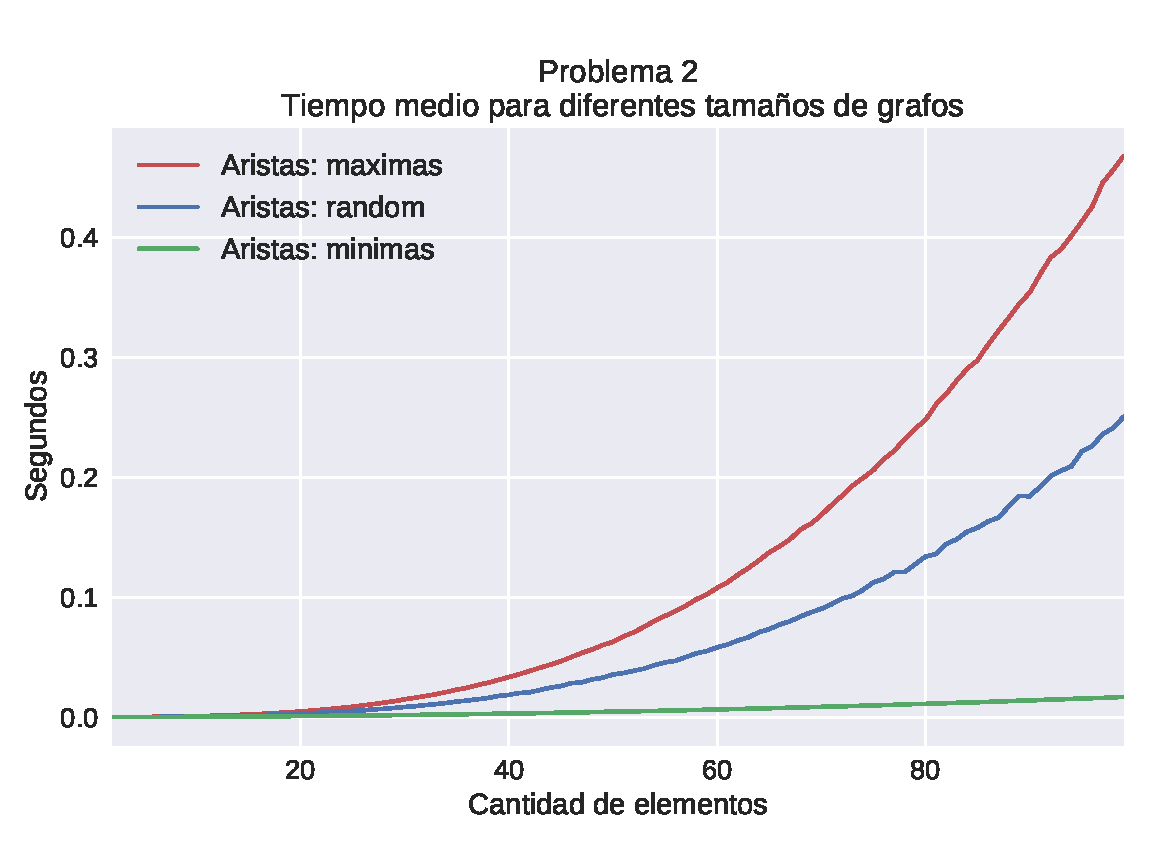
\includegraphics[width=0.8\textwidth]{imagenes/problema2/n_aristas.pdf} \\
}

Observemos que si las aristas son máximas, entonces $m = \frac{n*(n-1)}{2}$, con lo cual $O(n*m) = O(n^3)$. Además, la esperanza de la cantidad de aristas tomadas al azar sería $m = \frac{n*(n-1)}{4}$, con lo cual seguiría siendo de orden cúbico. Estos hechos parecerían corresponderse con lo que vemos en el gráfico. \\

Algo interesante que podemos notar es el hecho de que las funciones sean tan suaves como lo son. Recordar que en un algoritmo de Ford común se tienen condiciones de corte (podría detenerse si en una iteración no hay cambios). Esto no ocurre en este caso porque lo estamos utilizando para detectar ciclos negativos, con lo cual siempre iteramos $n+1$ veces. Además, a Ford no le interesa mucho la topología de nuestros grafos, porque en cada iteración termina visitando todas las aristas, independientemente de qué es lo que estén conectando. Cómo resultado, no hay nada más que pueda afectar el recorrido del algoritmo que las variables presentes en la fórmula planteada en la sección de Complejidad.